\documentclass{article}
\usepackage[utf8]{inputenc}
\usepackage{graphicx}
\usepackage{hyperref}

\title{ASSIGNMENT 1 NEURAL NETWORKS: SUPERVISED LEARNING}
\author{Ismael Peruga, Álvaro González}
\date{January 2017}

\begin{document}

\maketitle
\section{Introduction}
In this first assignment, the k-NN and backpropagation algorithms have to be implemented. To see the performance of this algorithms we are given 4 different sets of data, with different features number and distributions.

\section{Data}
To perform this assignment, 4 different sets of data are given. The first 3 consists of 2-dimensional features (the first and the second have 2 classes and the third have 3), the 4th is composed with OCR digits that have 64 features and 10 different classes (from 0 to 9).

\subsection{Set data 1}
In the first set of data it is clearly seen that the 2 classes are linearly separable since in the vertical dimension (see figure \ref{fig:dataset1}) there is not a great overlap.
\begin{figure}[!htb]
\centering
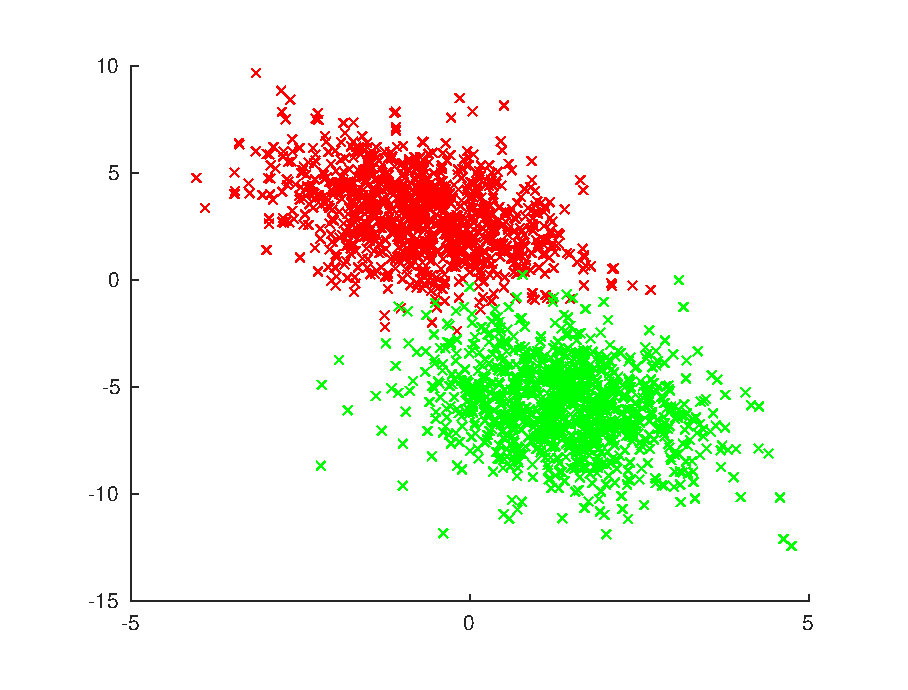
\includegraphics[height=4cm]{images/dataset1}
\caption{Dataset 1}
\label{fig:dataset1}
\end{figure}

\subsection{Set data 2}
Regarding the second dataset, drawing a line that separates the 2 classes is impossible without commit a big error in the classification. This means that if we want to clasify correctly samples from this dataset, it is neccesary to use a non linear classifier. 
\begin{figure}[!htb]
\centering
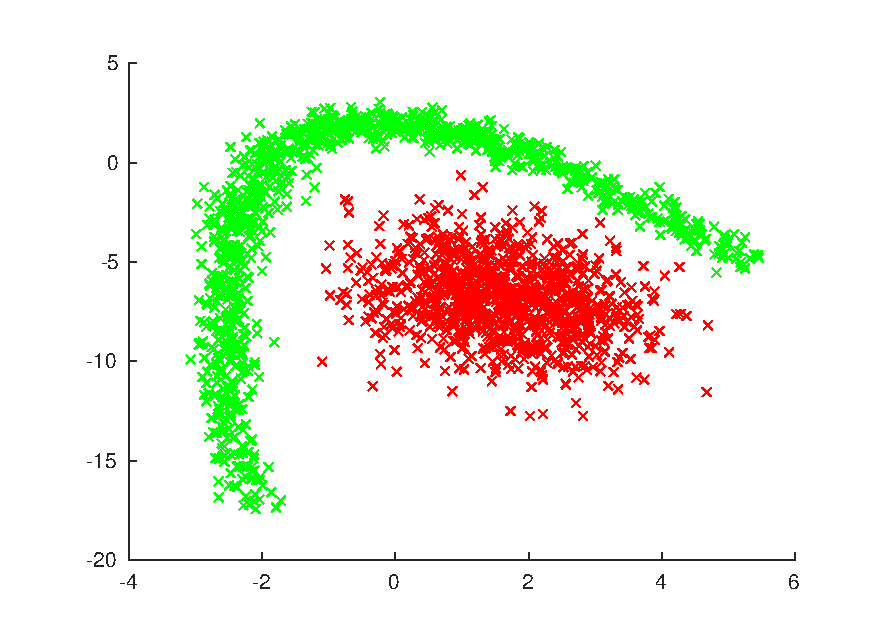
\includegraphics[height=4cm]{images/dataset2}
\caption{Dataset 2}
\label{fig:dataset2}
\end{figure}

\subsection{Set data 3}
The third set of data is more or less similar to the second, but in this case, there are 3 different classes and as for the second set they are not linearly separable. For this dataset it is also needed a non linear classifier to achieve good performance.
\begin{figure}[!htb]
\centering
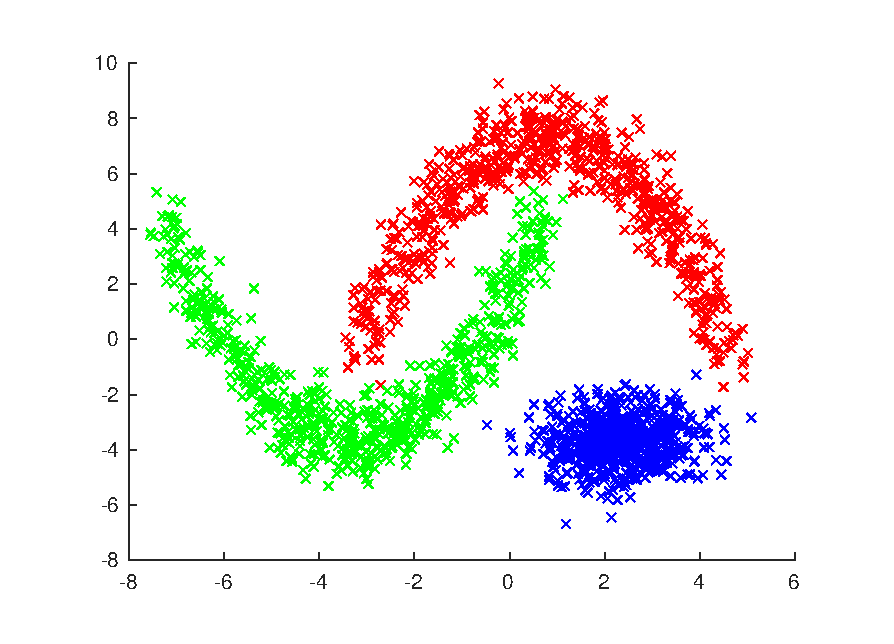
\includegraphics[height=4cm]{images/dataset3}
\caption{Dataset 3}
\label{fig:dataset3}
\end{figure}
\subsection{Set data 4}
This set of data is OCR. It represents handwritten numbers. Each element of this set has 64 different features (which are the 8x8 matrix, where each element is between the 0 and 16 range). This set has been down-sampled from 32x32 to 8x8 by dividing the big matrix in blocks of 4x4. It allows to reduce the dimensions and give less variance to small distortions. Since in this dataset the features are the value of each block in a gray scale, it is not linearly separable. 

\section{K-Nearest Neighbours (k-NN)}
In the first task, the k-NN algorithm has to be implemented. This is a method of classification which consist in a comparison of the input data and all the training examples. The output of this algorithm is the estimated class of the input data.

To implement this, the euclidean distance is calculated between all training data and the input. All these distances are stored in a vector and the k smallest distances are taking in account to decide the output class. It is a vote system where the winner is the class with more neighbours between the k-nearest. In case of draw, the algorithm takes the class that has the minimum accumulative distance (for example if there are 2 classes that have 2 elements between the k-nearest neighbours, the distances of each element of each class are added and the class with the minimum distance is selected).

\subsection{Best K for each dataset}
To find the optimal value of k in the different datasets, the cross validation technique has been implemented. First of all, the selected dataset is divided in a certain number of bins. Once it has been divided, one bin is used as test data and the remaining bins are used as training data. Then the bin used for testing is rotated until all bins have been used for testing. The accuracy result is the mean of the accuracy for each division of data (testing-training). This procedure is repeated for different values of k (in our case k goes from 1 to 50) and all is stored into a vector. Finally the best accuracy in this vector gives the optimal k.

To select the best K for each dataset we are dividing each dataset in 5 bins with 100 samples per class. 

\subsubsection {Best K for dataset 1}
For the first dataset, following the method explained before, we get a best K of 3 and 20, as both K give the same average accuracy of 0.993.

\begin{figure}[!htb]
\centering
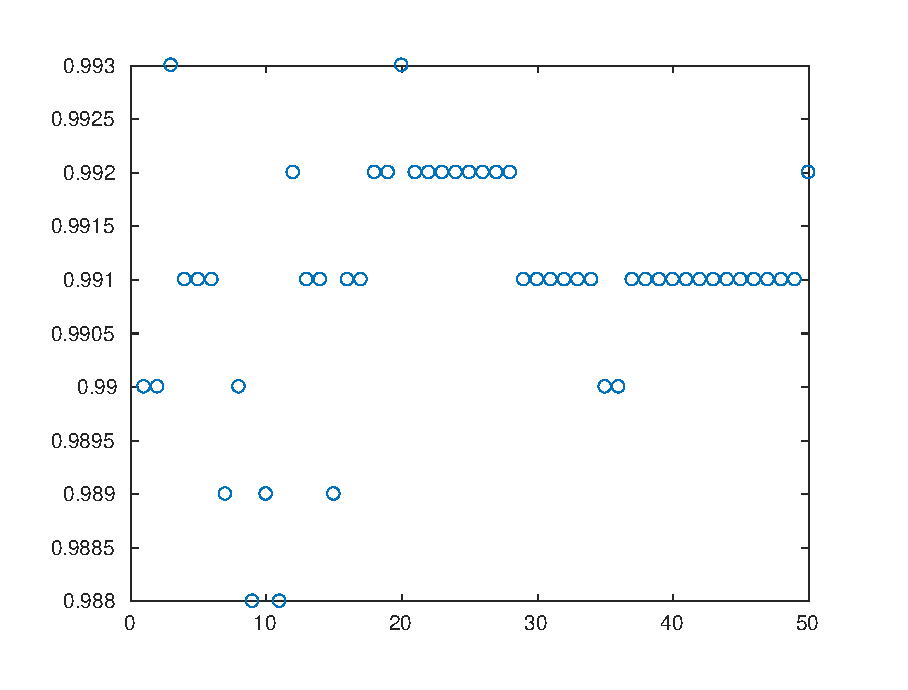
\includegraphics[height=4cm]{images/bestkdataset1}
\caption{Best K for dataset 1}
\label{fig:bestkdataset1}
\end{figure}

In the figure it can be seen the average accuracy for each k. In this case where is a draw between k=3 and k=20, the best choice is 3 as it will need less computational power than 20. For this data set, the worse accuracy is 0.988 where k is 9 or 11, which is still a good performance.

As an example, the output of the algorithm with k = 3 is the following:

\begin{figure}[!htb]
\centering
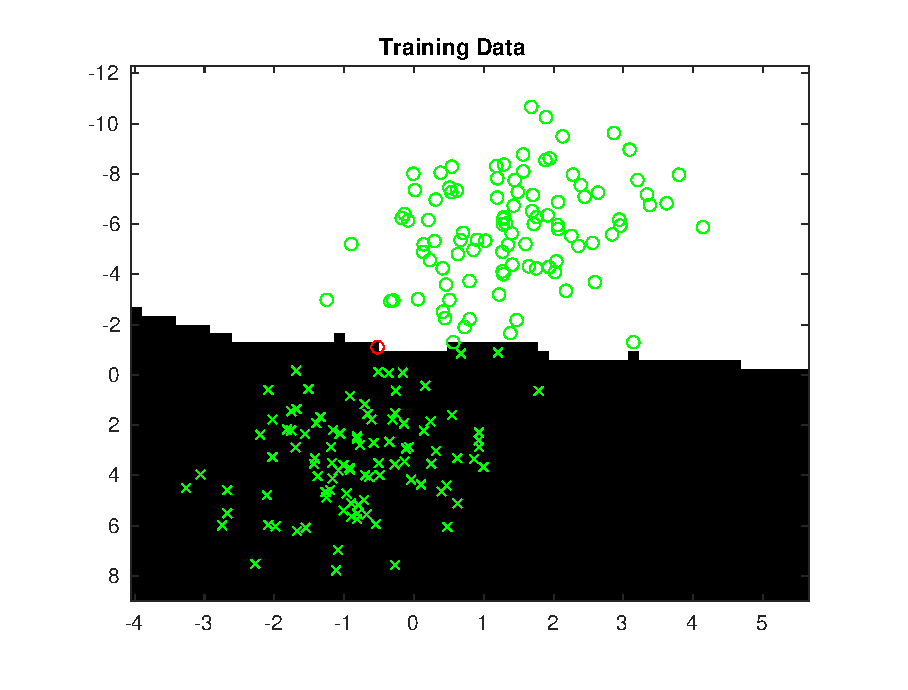
\includegraphics[height=4cm]{images/resultsknn1}
\caption{Output Example For Dataset 1}
\label{fig:resultsknn1}
\end{figure}


\subsubsection {Best K for dataset 2}
In the second dataset, the best K is 1 and 2, both produce an accuracy of 0.999.

\begin{figure}[!htb]
\centering
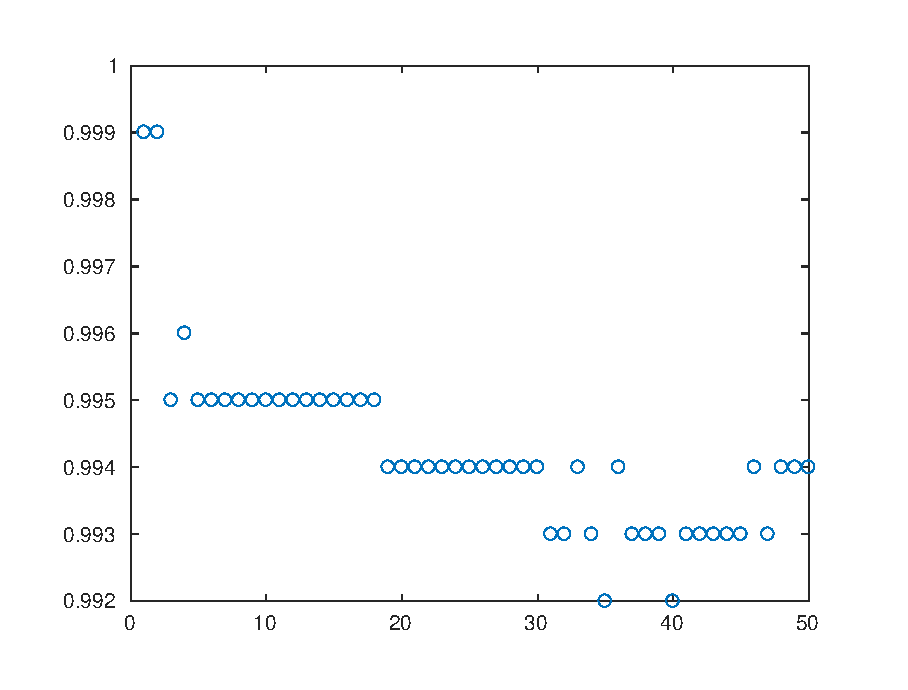
\includegraphics[height=4cm]{images/bestkdataset2}
\caption{Best K for dataset 2}
\label{fig:bestkdataset2}
\end{figure}

The example using k = 1 (see figure \ref{fig:resultsknn2}) :

\begin{figure}[!htb]
\centering
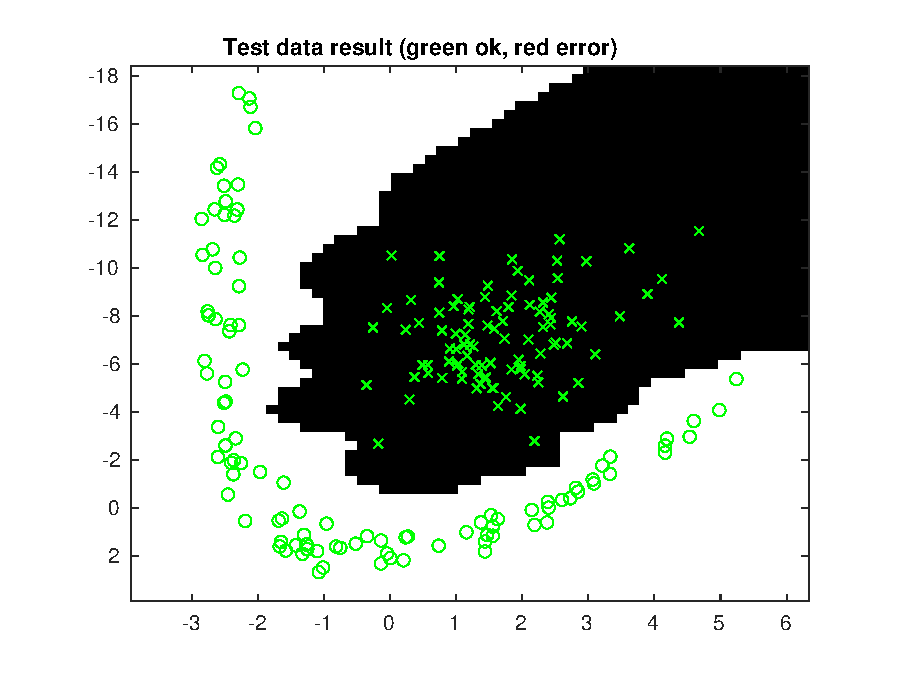
\includegraphics[height=4cm]{images/resultsknn2}
\caption{Output Example For Dataset 2}
\label{fig:resultsknn2}
\end{figure}


\subsubsection {Best K for dataset 3}
Regarding the third dataset, the best K is found to be 1, 3, 4 and 5. In this case it can be seen a pattern that if more neighbours are added, the performance is worse.

\begin{figure}[!htb]
\centering
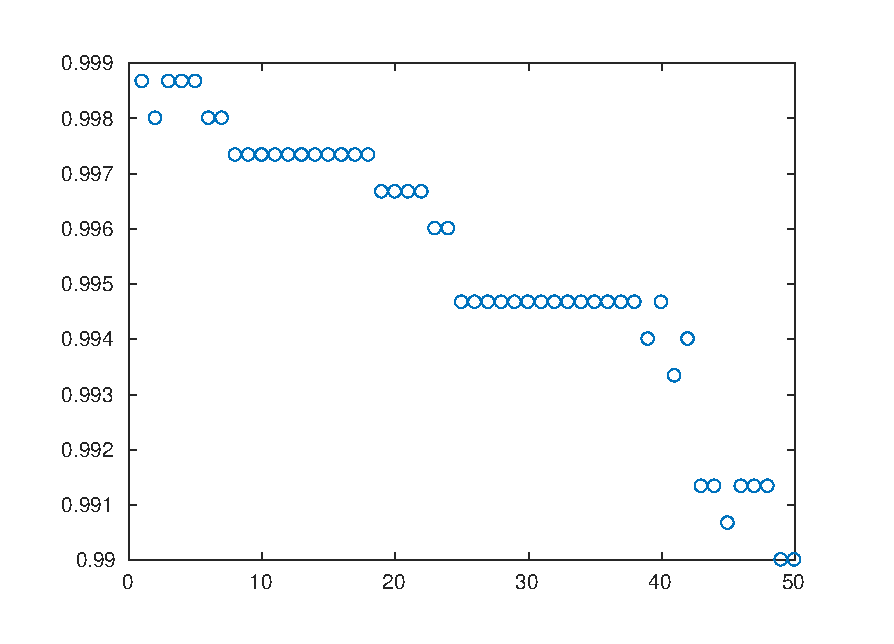
\includegraphics[height=4cm]{images/bestkdataset3}
\caption{Best K for dataset 3}
\label{fig:bestkdataset3}
\end{figure}

The example using k = 1 (see figure \ref{fig:resultsknn3}) :

\begin{figure}[!htb]
\centering
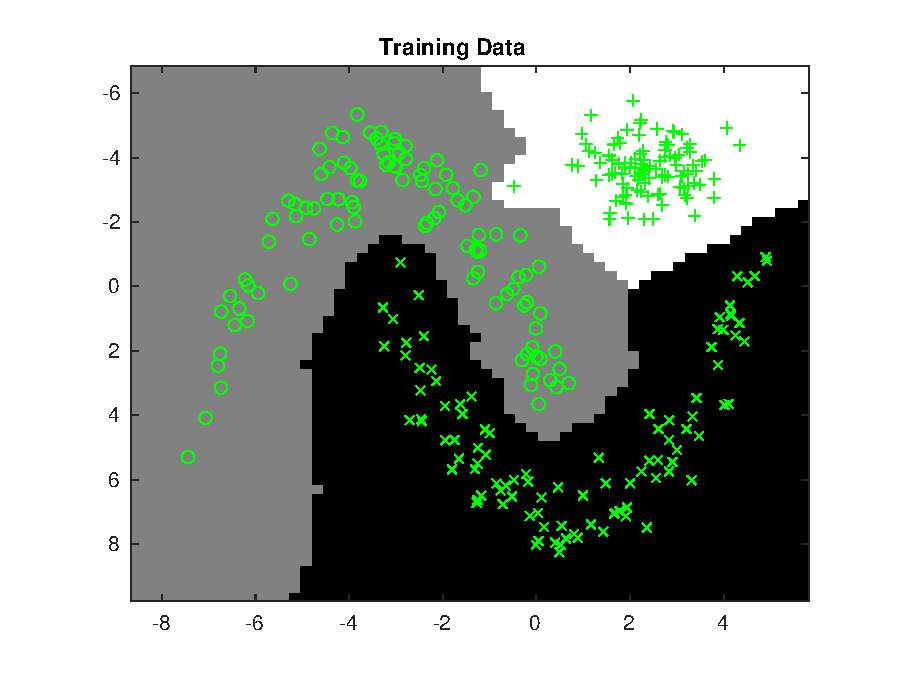
\includegraphics[height=4cm]{images/resultsknn3}
\caption{Output Example For Dataset 3}
\label{fig:resultsknn3}
\end{figure}

\subsubsection {Best K for dataset 4}
For the last dataset, the best K is 3 and there is no draw. It gives an accuracy of 0.9862. There is also worse performance whereas K is increasing.

\begin{figure}[!htb]
\centering
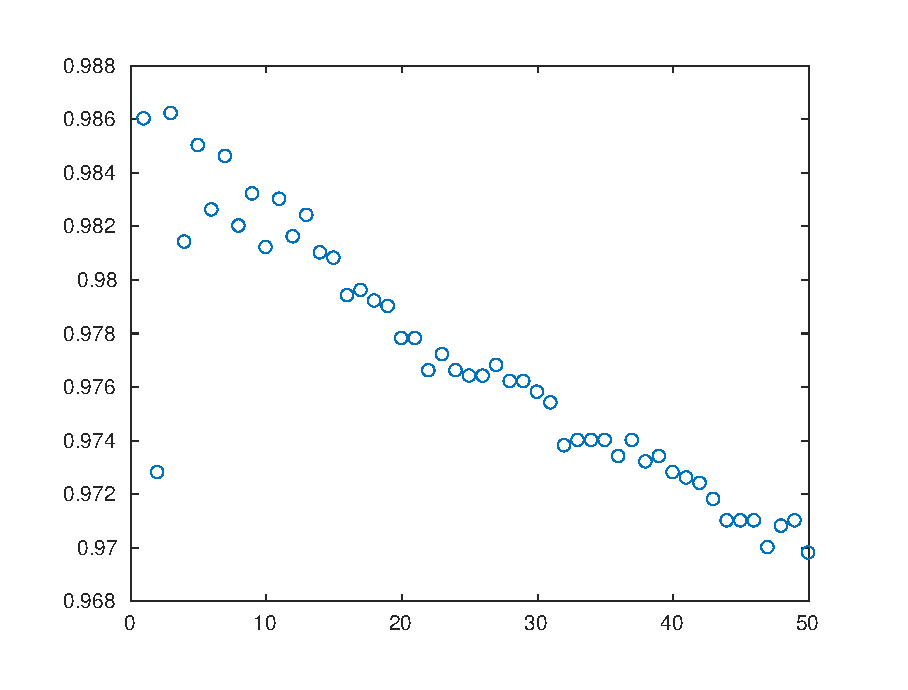
\includegraphics[height=4cm]{images/bestkdataset4}
\caption{Best K for dataset 4}
\label{fig:bestkdataset4}
\end{figure}

The example using k = 3 (see figure \ref{fig:resultsknn4}) :

\begin{figure}[!htb]
\centering
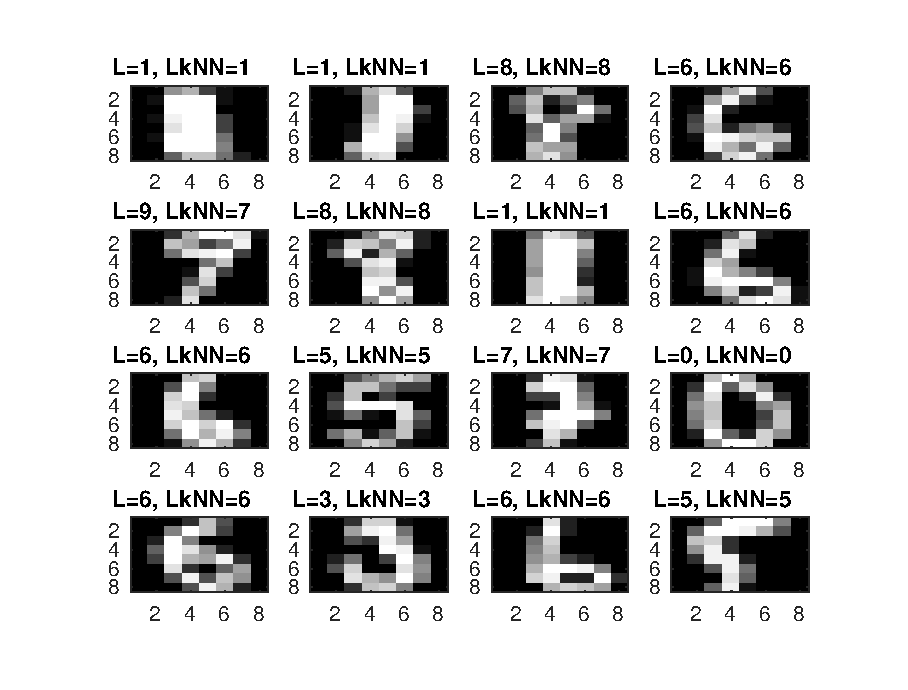
\includegraphics[height=4cm]{images/resultsknn4}
\caption{Output Example For Dataset 4}
\label{fig:resultsknn4}
\end{figure}




\section{Backpropagation}
A neural network is a set of layers that contains nonlinear functions (called activation functions). The inputs of these functions are the weighted sums of the outputs of the previous layer (or the system input for the first layer). The final layer gives the output of the network. 

The weighted sums $\mathbf{z}^{(l)}$ of layer $l$ are calculated multiplying the weights' matrix $\mathbf{W}^{(l)}$ of layer $l$ by the activation vector $\mathbf{a}^{(l-1)}$ of the layer $l-1$:

$$\mathbf{z}^{(l)} = \mathbf{W}^{(l)}\mathbf{a}^{(l-1)}$$

We are adding a bias unit with constant value to the activation vectors to let the separating hyperplane move from the origin. Then we apply the activation function $\sigma$ on the resulting values to obtain the activation vector of that layer. The activation function we used is the hiperbolic tangent, that maps to the interval $(-1,1)$ and is differentiable.

$$\mathbf{a}^{(l)} = \sigma(\mathbf{z}^{(l)}) = \tanh(\mathbf{z}^{(l)})$$

Learning occurs by adjusting the weights between layers. All the operations in a neural network are differentiable, so we can calculate the gradient of the cost function respect of the weights $\frac{\partial C}{\partial \mathbf{W}^{(l)}}$. We use this to reduce the classification error by iteratively moving the weights with small steps in the opposite direction of the gradient. We use batch learning to have a more stable learning.




\subsection{Single Layer Neural Network}

In this model we only have one layer of weights. In fact, we don't even need to apply the activation function, as we are only interested in the output class with the maximum value. The activation of the output layer $\mathbf{a}$ is then

$$\mathbf{a} = \mathbf{W}\mathbf{x}$$

where $\mathbf{x}$ is the input.

The gradient is calculated by

$$\frac{\partial C}{\partial \mathbf{W}} = \frac{2}{N} \left ( \mathbf{a} - \mathbf{y} \right ) \mathbf{x}^T$$

where $N$ is the number of samples in the batch and $\mathbf{y}$ is the correct output. Then we update the weights with

$$\mathbf{W} \leftarrow \mathbf{W} - \varepsilon \frac{\partial C}{\partial \mathbf{W}}$$

where $\varepsilon$ is the learning rate, with a typical value around $10^{-5}$.


\subsection{Multiple Layer Neural Network}

In this model we are using two layers. The \textbf{gradient in the second layer} is calculated with

$$\frac{\partial C}{\partial \mathbf{W}^{(2)}} = \mathbf{\delta}^{(2)} {\mathbf{a}^{(1)}}^T$$

where $\mathbf{\delta}^{(l)}$ is the error vector in layer $l$. In layer 2 it is calculated by

$$\mathbf{\delta}^{(2)} = (\mathbf{a}^{(2)} - \mathbf{y}) \odot \tanh'\left (\mathbf{z}^{(2)} \right )$$

where $\odot$ is an element-wise multiplication. The \textbf{gradient in the first layer} is

$$\frac{\partial C}{\partial \mathbf{W}^{(1)}} = \mathbf{\delta}^{(1)} {\mathbf{x}}^T$$

and the error vector in layer 1 is calculated by

$$\mathbf{\delta}^{(1)} = {\mathbf{W}^{(2)}}^T\mathbf{\delta}^{(2)} \odot \tanh'\left (\mathbf{z}^{(1)} \right )$$

We are using error vectors in our equations (as seen \href{http://neuralnetworksanddeeplearning.com/}{\textit{here}}) because this simplifies a lot the expressions and the calculations. 

Finally, we update the weights with

$$\mathbf{W}^{(2)} \leftarrow \mathbf{W}^{(2)} - \varepsilon \frac{\partial C}{\partial \mathbf{W}^{(2)}}$$
$$\mathbf{W}^{(1)} \leftarrow \mathbf{W}^{(1)} - \varepsilon \frac{\partial C}{\partial \mathbf{W}^{(1)}}$$

We added a technique called momentum to have a faster convergence. This technique consists in add part of the previous change of weights to the next change of weights. We have seen that this technique can be useful with complex datasets, like the OCR dataset.

\subsection{Results}

\subsubsection{Single Layer Neural Network}

With this model we only get the asked results in the dataset 1, the linearly separable one. The accuracy in the others is not good enough.

In dataset 1 we obtained an accuracy of 0.9950 with 400 iterations and 0.005 as learning rate. We show here the learning curve (see figure \ref{fig:single_data1_error}) and training (figure \ref{fig:single_data1_result_train}) and test results (figure \ref{fig:single_data1_result_test}).

\begin{figure}[!htb]
\centering
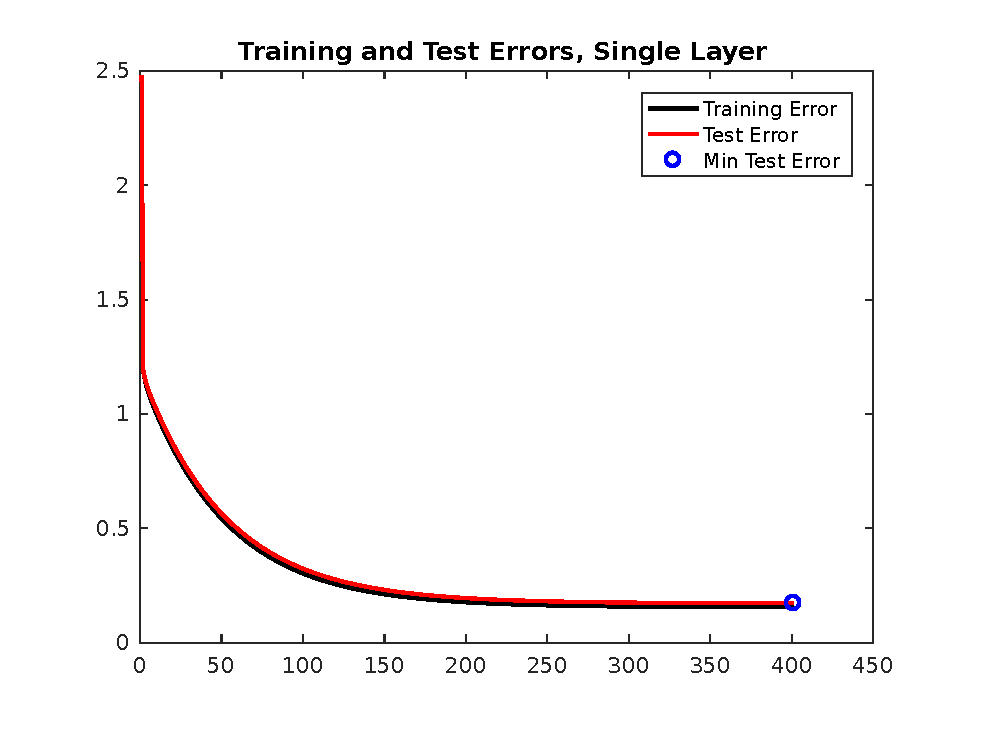
\includegraphics[height=4cm]{images/single_data1_error}
\caption{Error curve of a single layered neural network in the dataset 1.}
\label{fig:single_data1_error}
\end{figure}

\begin{figure}[!htb]
\centering
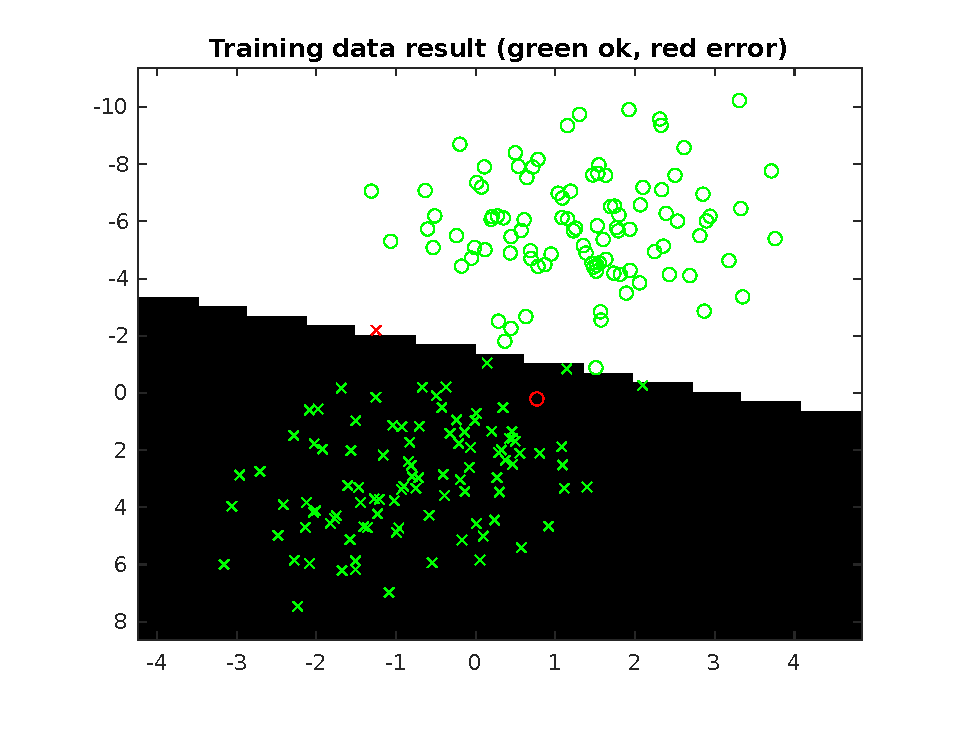
\includegraphics[height=4cm]{images/single_data1_result_train}
\caption{Results of a single layered neural network in the training set 1.}
\label{fig:single_data1_result_train}
\end{figure}

\begin{figure}[!htb]
\centering
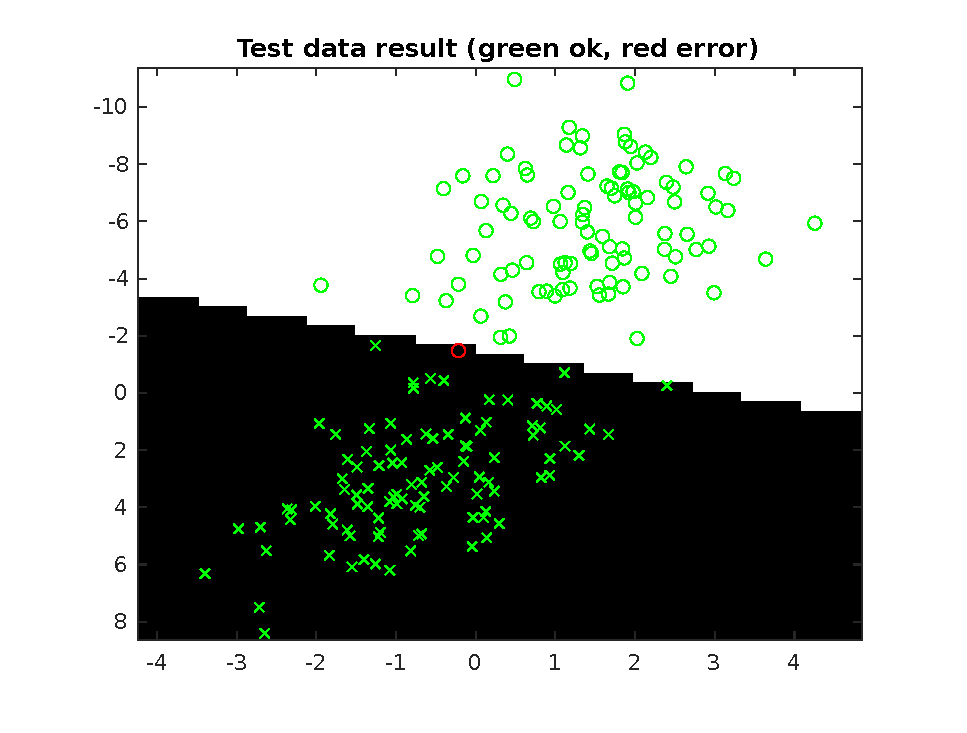
\includegraphics[height=4cm]{images/single_data1_result_test}
\caption{Results of a single layered neural network in the test set 1.}
\label{fig:single_data1_result_test}
\end{figure}


In dataset 2 we obtained an accuracy of 0.8300 with 400 iterations and 0.005 as learning rate. We show here the learning curve (see figure \ref{fig:single_data2_error}) and training (figure \ref{fig:single_data2_result_train}) and test results (figure \ref{fig:single_data2_result_test}).

\begin{figure}[!htb]
\centering
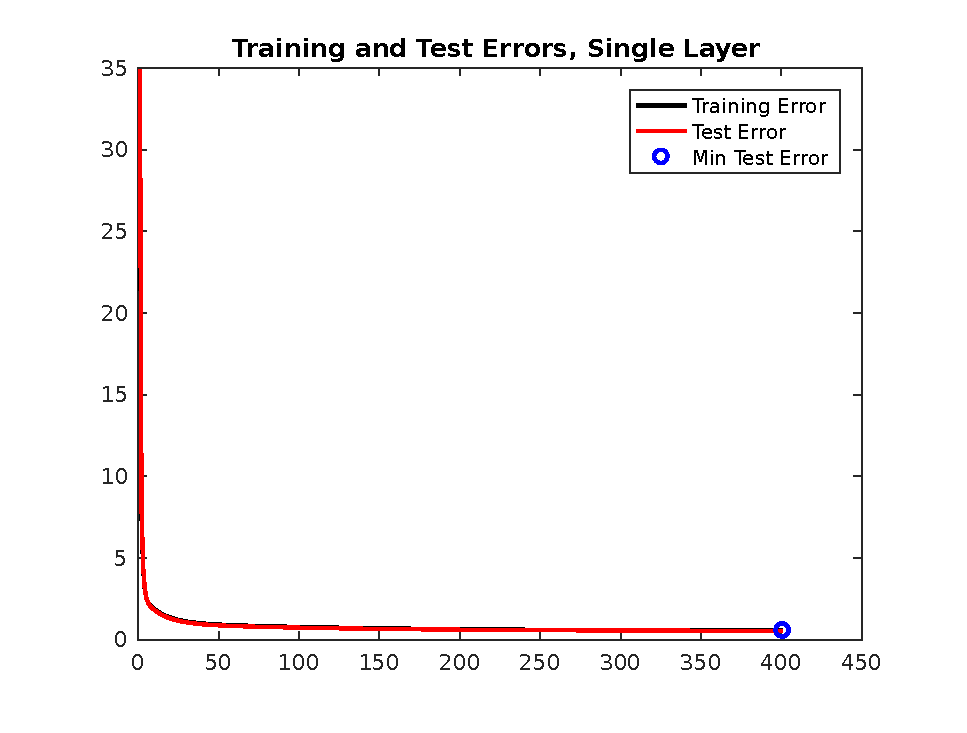
\includegraphics[height=4cm]{images/single_data2_error}
\caption{Error curve of a single layered neural network in the dataset 2.}
\label{fig:single_data2_error}
\end{figure}

\begin{figure}[!htb]
\centering
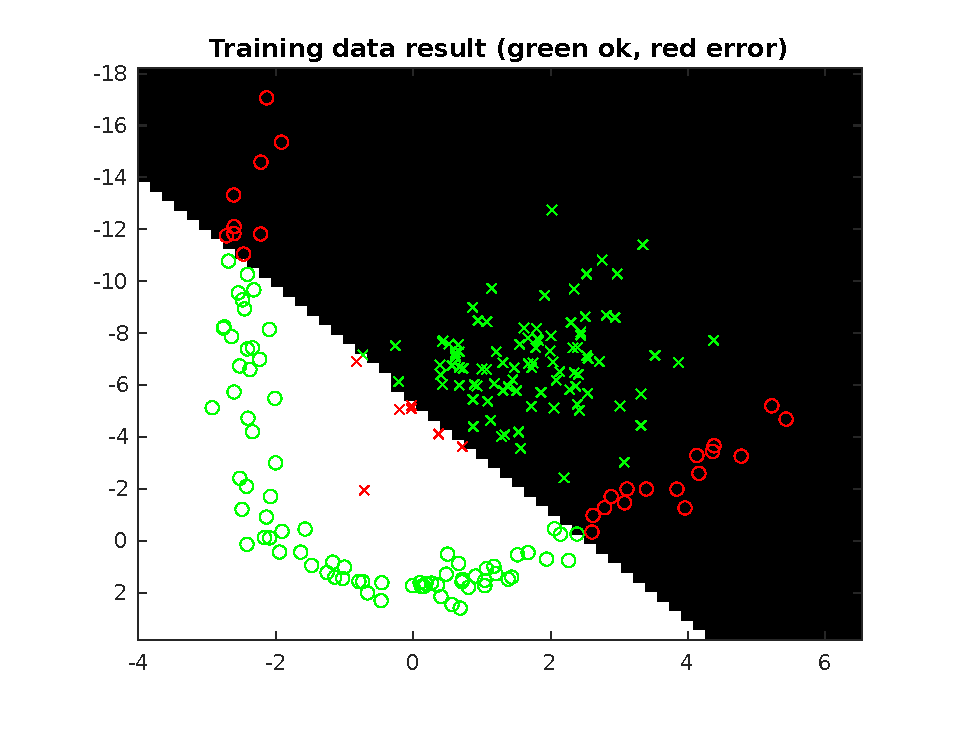
\includegraphics[height=4cm]{images/single_data2_result_train}
\caption{Results of a single layered neural network in the training set 2.}
\label{fig:single_data2_result_train}
\end{figure}

\begin{figure}[!htb]
\centering
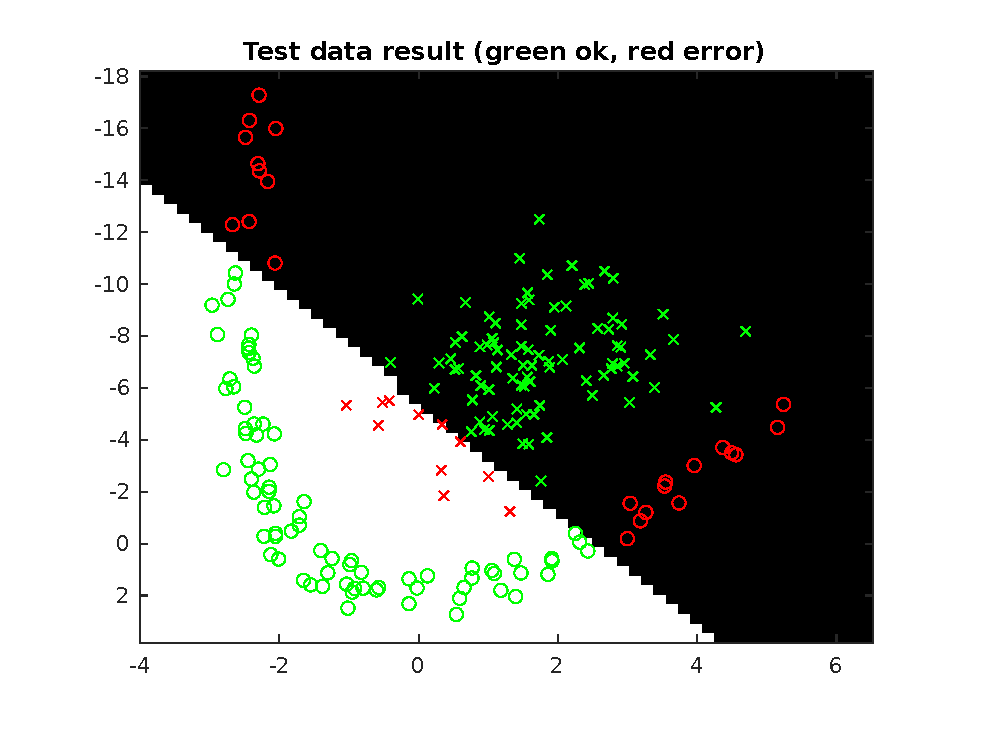
\includegraphics[height=4cm]{images/single_data2_result_test}
\caption{Results of a single layered neural network in the test set 2.}
\label{fig:single_data2_result_test}
\end{figure}


In dataset 3 we obtained an accuracy of 0.9000 with 400 iterations and 0.005 as learning rate. We show here the learning curve (see figure \ref{fig:single_data3_error}) and training (figure \ref{fig:single_data3_result_train}) and test results (figure \ref{fig:single_data3_result_test}).

\begin{figure}[!htb]
\centering
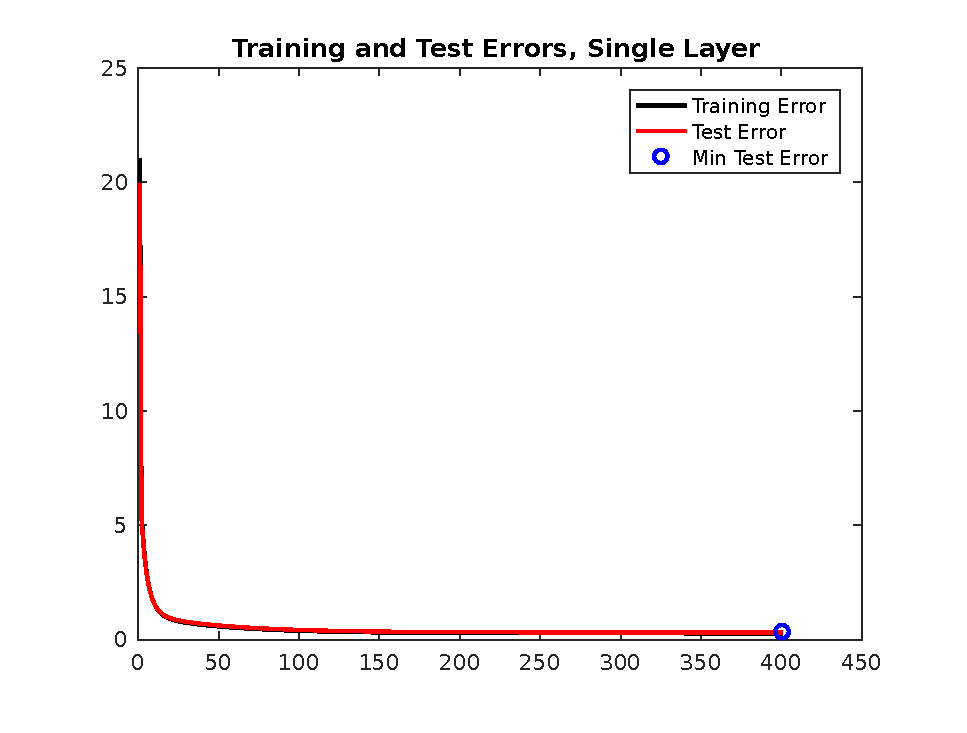
\includegraphics[height=4cm]{images/single_data3_error}
\caption{Error curve of a single layered neural network in the dataset 3.}
\label{fig:single_data3_error}
\end{figure}

\begin{figure}[!htb]
\centering
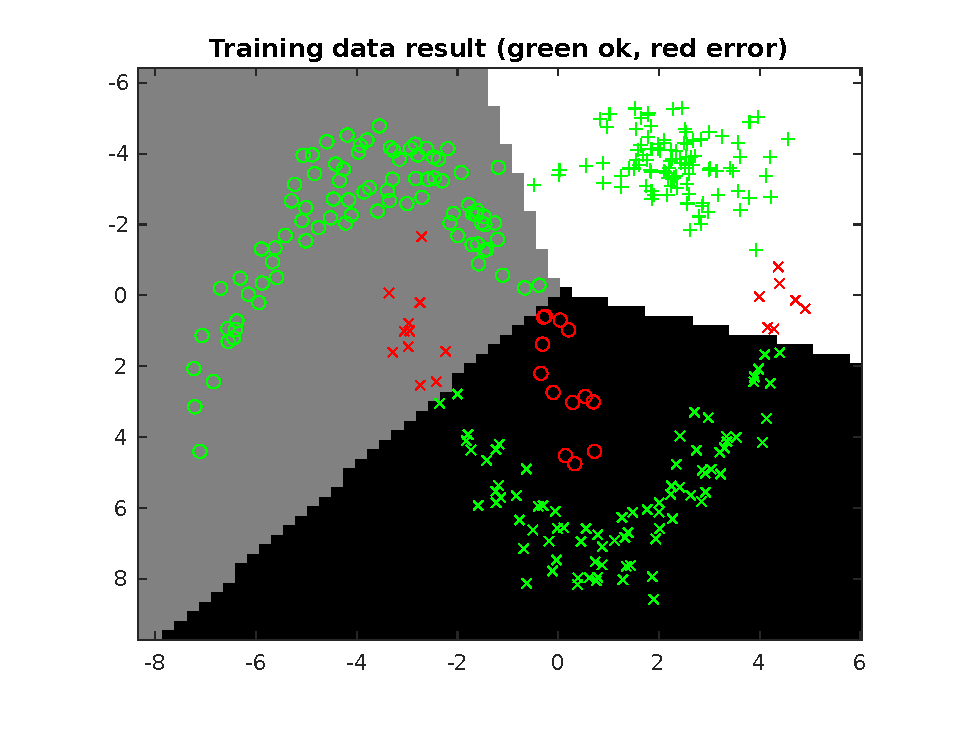
\includegraphics[height=4cm]{images/single_data3_result_train}
\caption{Results of a single layered neural network in the training set 3.}
\label{fig:single_data3_result_train}
\end{figure}

\begin{figure}[!htb]
\centering
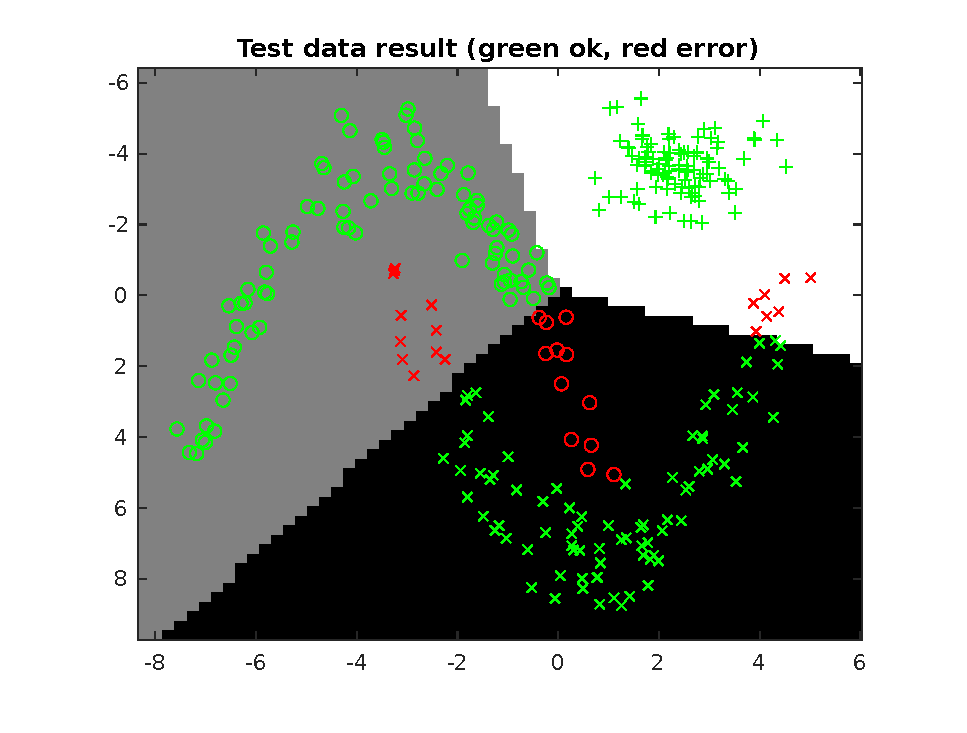
\includegraphics[height=4cm]{images/single_data3_result_test}
\caption{Results of a single layered neural network in the test set 3.}
\label{fig:single_data3_result_test}
\end{figure}


In dataset 4, we saw that learning doesn't finish to settle with few iterations, so when we set much more we obtain good results. We used $5*10^4$ iterations and $1*10^{-4}$ as learning rate, obtaining an accuracy of 0.9240.

\begin{figure}[!htb]
\centering
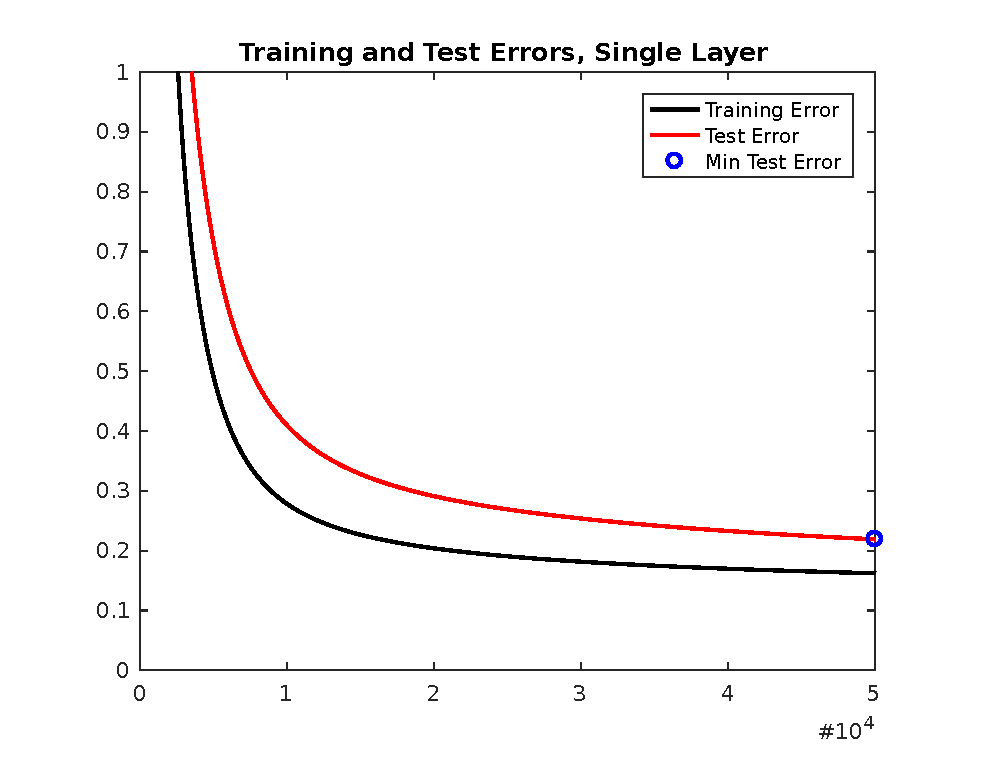
\includegraphics[height=4cm]{images/single_data4_error}
\caption{Error curve of a single layered neural network in the dataset 4.}
\label{fig:single_data4_error}
\end{figure}

\begin{figure}[!htb]
\centering
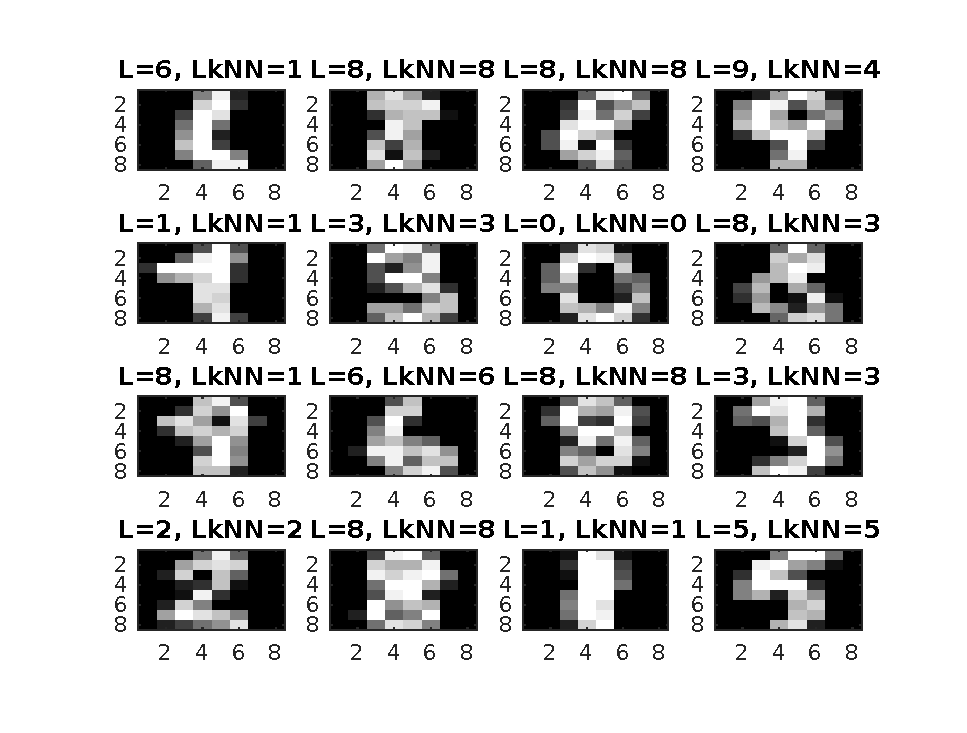
\includegraphics[height=4cm]{images/single_data4_result}
\caption{Results of a single layered neural network in the dataset 4.}
\label{fig:single_data4_result}
\end{figure}


\subsubsection{Multilayer Neural Network}

In dataset 1 we obtained an accuracy of 0.9950 with 4 hidden units, 100 iterations, 0.001 as learning rate and 0 momentum. We show here the learning curve (see figure \ref{fig:multi_data1_error}) and training (figure \ref{fig:multi_data1_result_train}) and test results (figure \ref{fig:multi_data1_result_test}).

\begin{figure}[!htb]
\centering
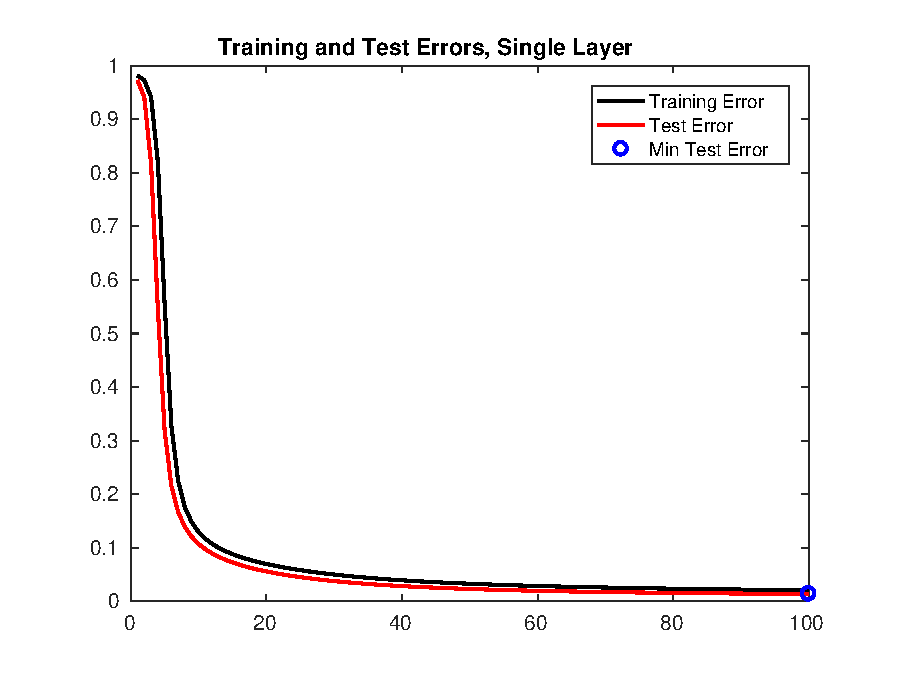
\includegraphics[height=4cm]{images/multi_data1_error}
\caption{Error curve of a multilayered neural network in the dataset 1.}
\label{fig:multi_data1_error}
\end{figure}

\begin{figure}[!htb]
\centering
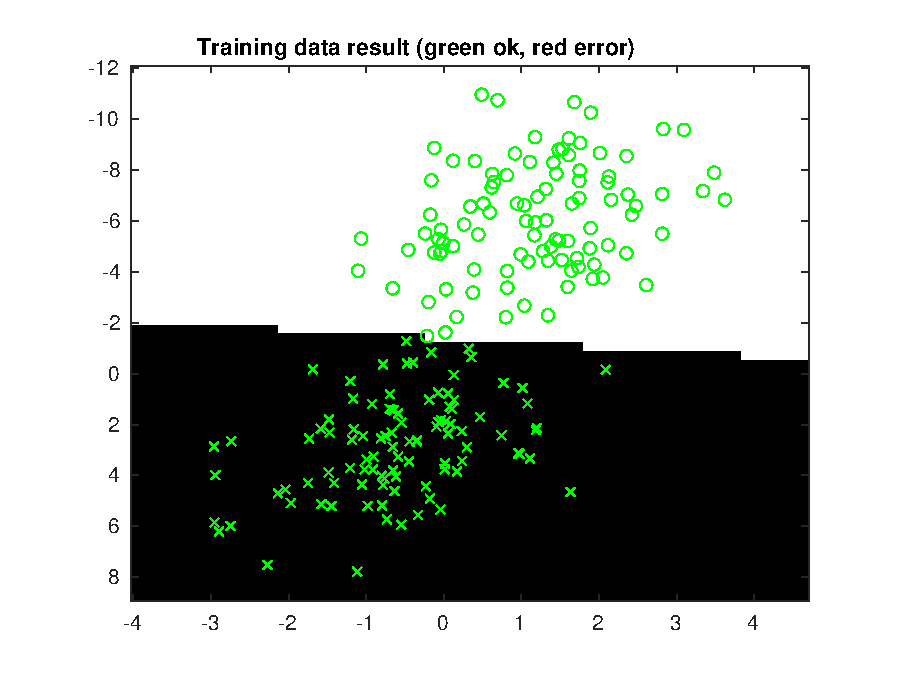
\includegraphics[height=4cm]{images/multi_data1_result_train}
\caption{Results of a multilayered neural network in the training set 1.}
\label{fig:multi_data1_result_train}
\end{figure}

\begin{figure}[!htb]
\centering
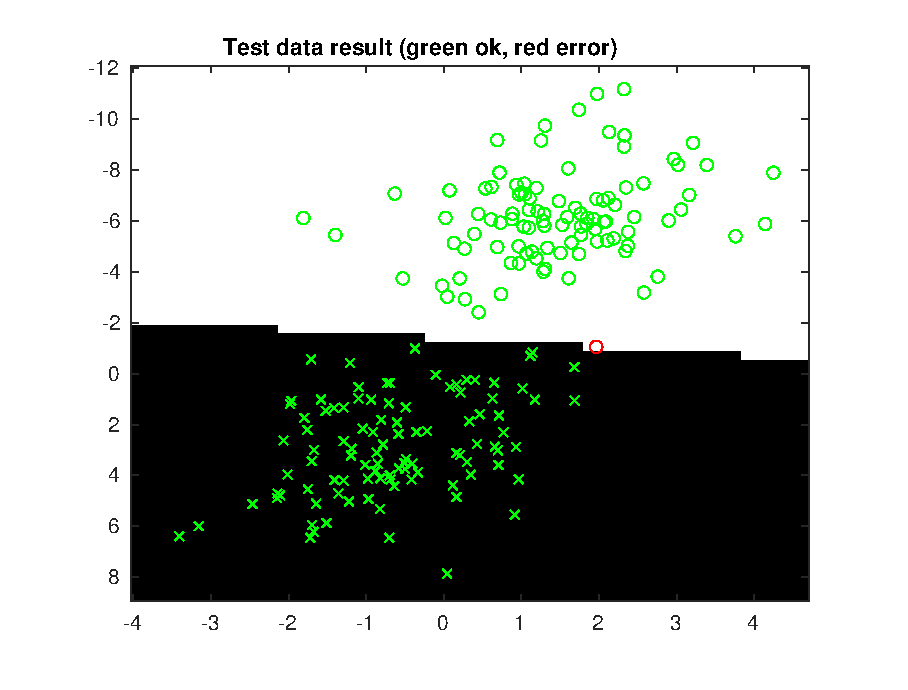
\includegraphics[height=4cm]{images/multi_data1_result_test}
\caption{Results of a multilayered neural network in the test set 1.}
\label{fig:multi_data1_result_test}
\end{figure}


In dataset 2 we obtained an accuracy of 0.9950 with 20 hidden units, 10000 iterations, 0.0001 as learning rate and 0 momentum. We show here the learning curve (see figure \ref{fig:multi_data2_error}) and training (figure \ref{fig:multi_data2_result_train}) and test results (figure \ref{fig:multi_data2_result_test}).

\begin{figure}[!htb]
\centering
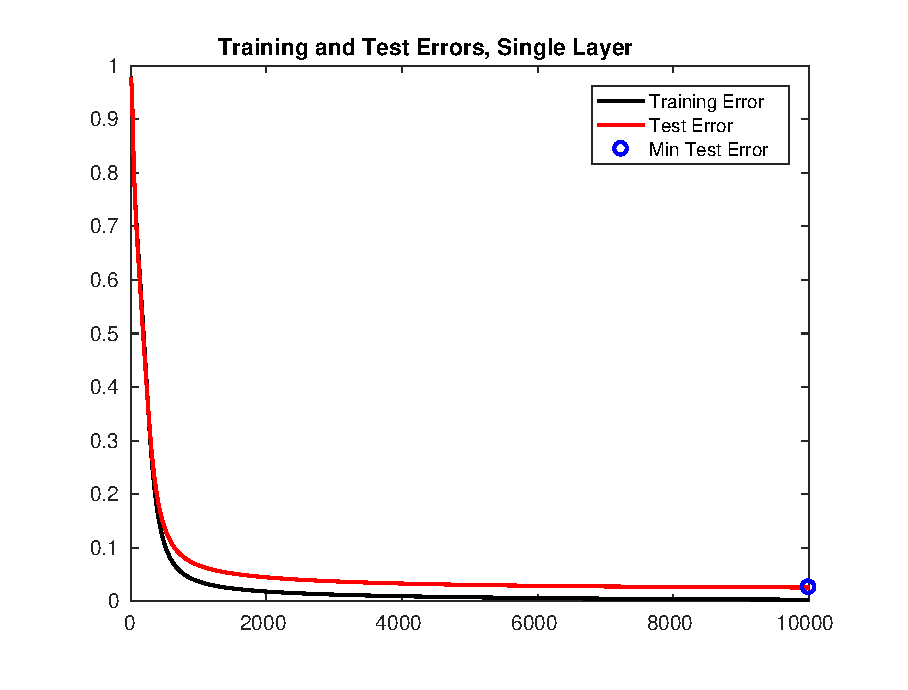
\includegraphics[height=4cm]{images/multi_data2_error}
\caption{Error curve of a multilayered neural network in the dataset 2.}
\label{fig:multi_data2_error}
\end{figure}

\begin{figure}[!htb]
\centering
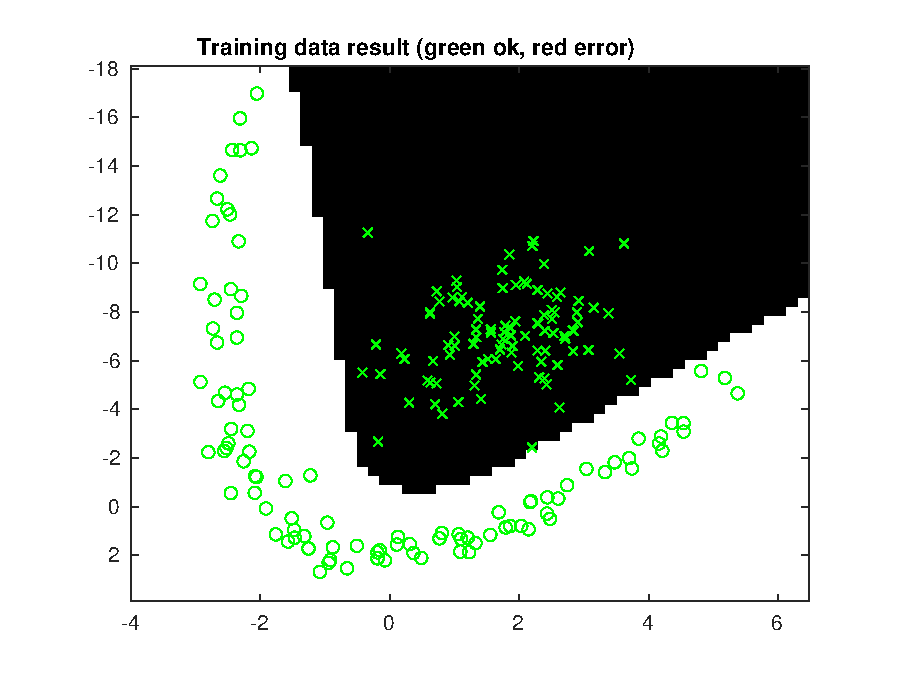
\includegraphics[height=4cm]{images/multi_data2_result_train}
\caption{Results of a multilayered neural network in the training set 2.}
\label{fig:multi_data2_result_train}
\end{figure}

\begin{figure}[!htb]
\centering
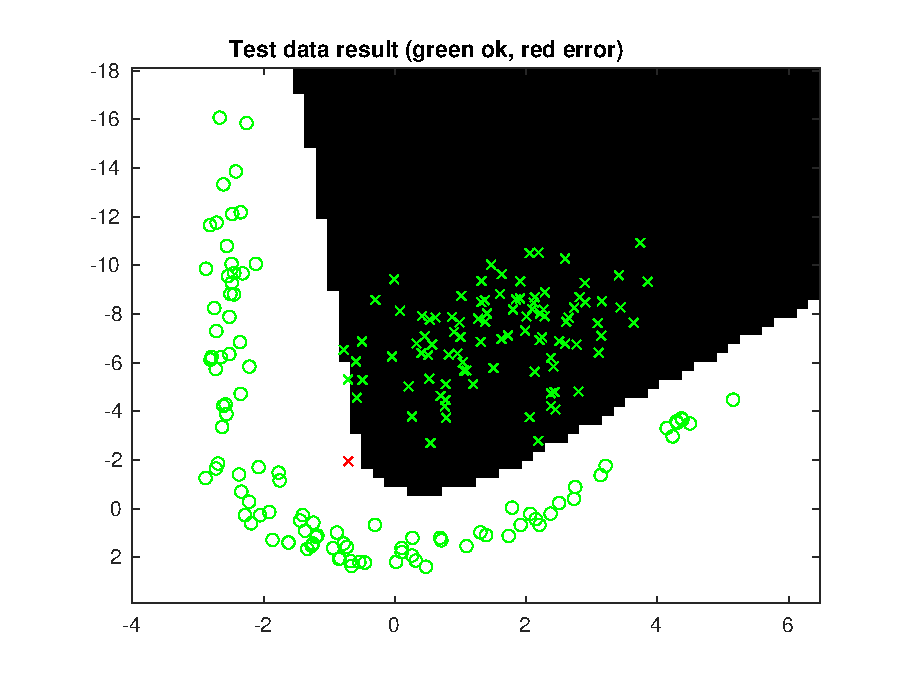
\includegraphics[height=4cm]{images/multi_data2_result_test}
\caption{Results of a multilayered neural network in the test set 2.}
\label{fig:multi_data2_result_test}
\end{figure}


In dataset 3 we obtained an accuracy of 0.9933 with 10 hidden units, 20000 iterations, 0.0001 as learning rate and 0 momentum. We show here the learning curve (see figure \ref{fig:multi_data3_error}) and training (figure \ref{fig:multi_data3_result_train}) and test results (figure \ref{fig:multi_data3_result_test}).

\begin{figure}[!htb]
\centering
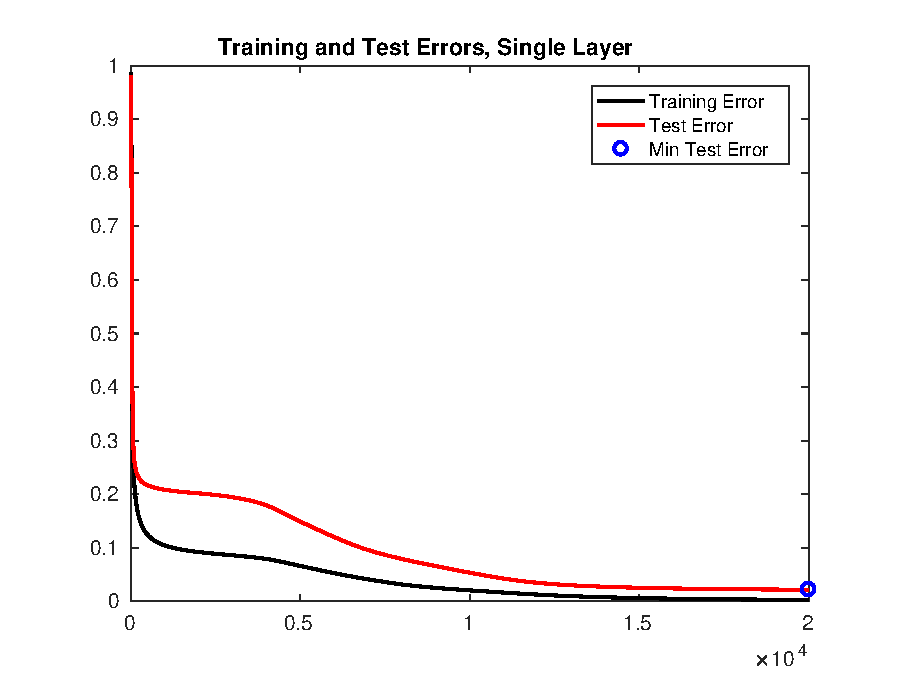
\includegraphics[height=4cm]{images/multi_data3_error}
\caption{Error curve of a multilayered neural network in the dataset 3.}
\label{fig:multi_data3_error}
\end{figure}

\begin{figure}[!htb]
\centering
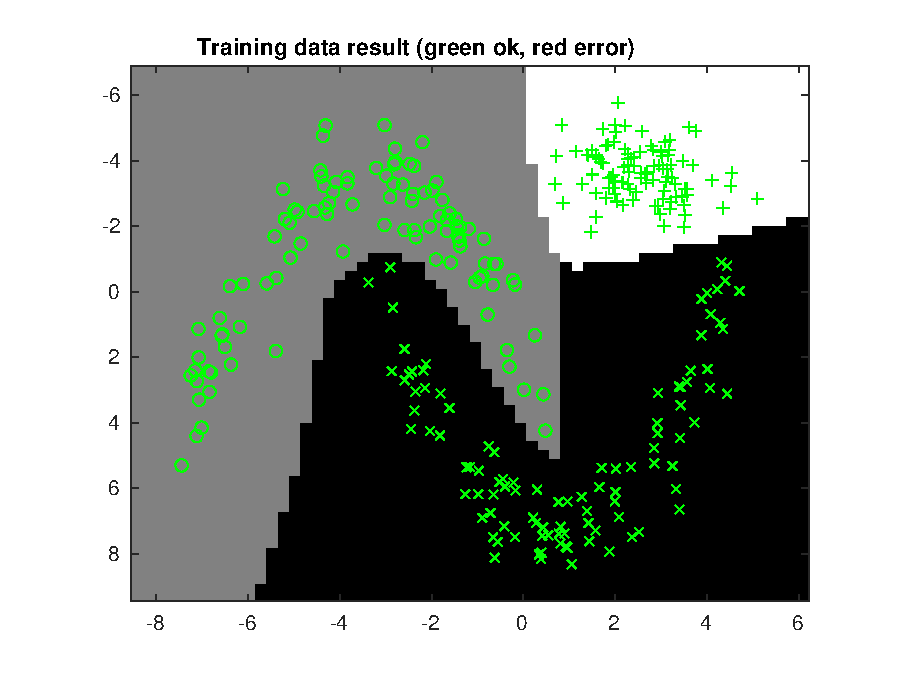
\includegraphics[height=4cm]{images/multi_data3_result_train}
\caption{Results of a multilayered neural network in the training set 3.}
\label{fig:multi_data3_result_train}
\end{figure}

\begin{figure}[!htb]
\centering
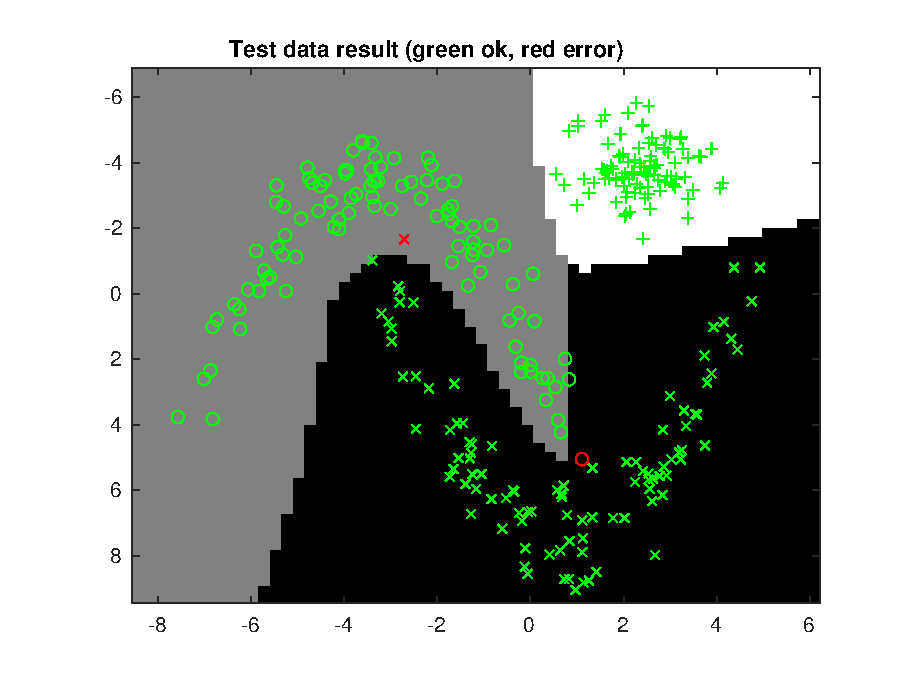
\includegraphics[height=4cm]{images/multi_data3_result_test}
\caption{Results of a multilayered neural network in the test set 3.}
\label{fig:multi_data3_result_test}
\end{figure}


In dataset 4 we obtained an accuracy of 0.9670 with 400 hidden units, 10000 iterations, 0.00001 as learning rate and 0.99 momentum. We show here the learning curve (see figure \ref{fig:multi_data4_error}) and some samples (figure \ref{fig:multi_data4_result}).

\begin{figure}[!htb]
\centering
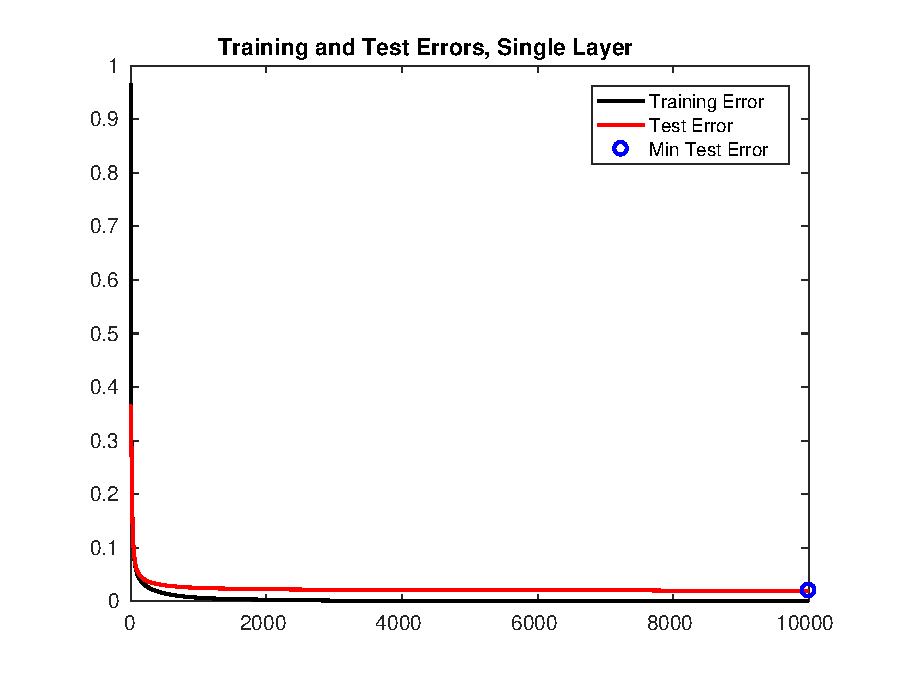
\includegraphics[height=4cm]{images/multi_data4_error}
\caption{Error curve of a multilayered neural network in the dataset 4.}
\label{fig:multi_data4_error}
\end{figure}

\begin{figure}[!htb]
\centering
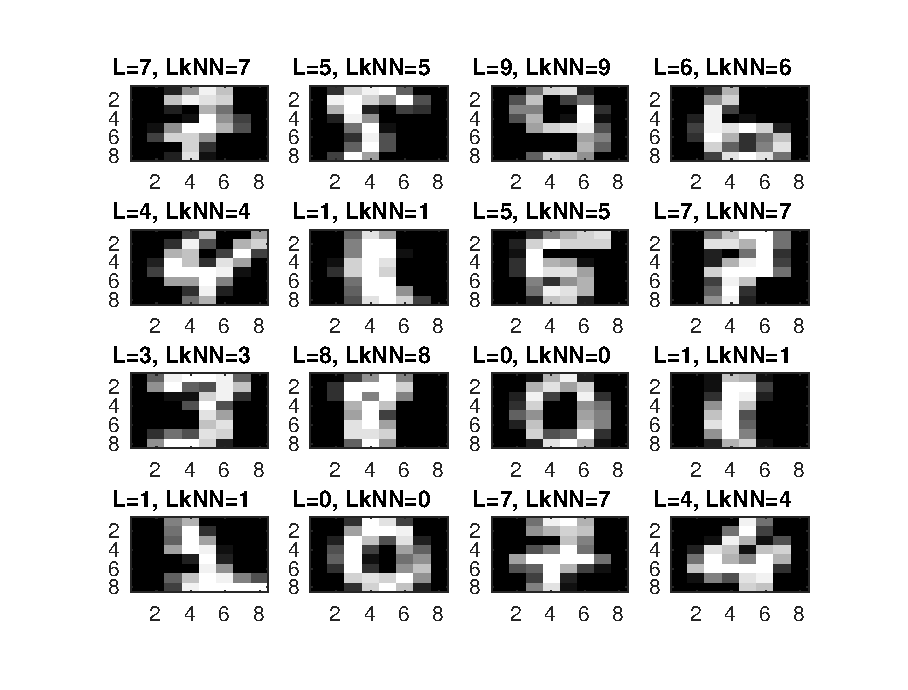
\includegraphics[height=4cm]{images/multi_data4_result}
\caption{Results of a multilayered neural network in the dataset 4.}
\label{fig:multi_data4_result}
\end{figure}


\subsection{Non-generalisable example}

We used a bin size of 5 samples, 200 hidden units, 10000 iterations, a learning rate of 0.01 and 0 momentum. With this ill configuration we obtained a very overfitted system, as can be easily seen in the learning curve (see figure \ref{fig:overfit_error}) and training (figure \ref{fig:overfit_result_train}) and test results (figure \ref{fig:overfit_result_test})

\begin{figure}[!htb]
\centering
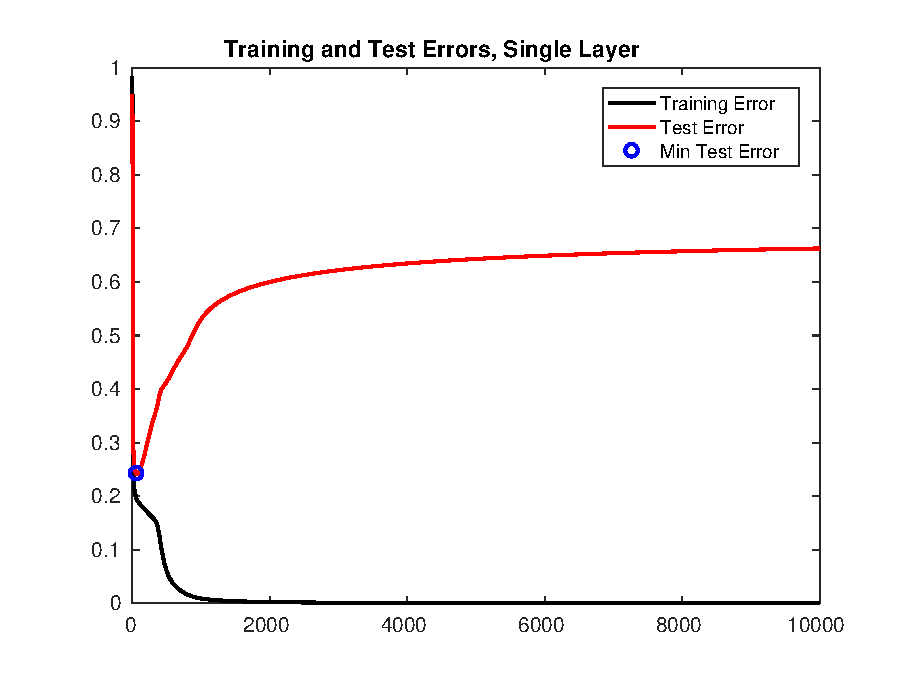
\includegraphics[height=4cm]{images/overfit_error}
\caption{Error curve of a multilayered neural network in a reduced version of the dataset 3.}
\label{fig:overfit_error}
\end{figure}

\begin{figure}[!htb]
\centering
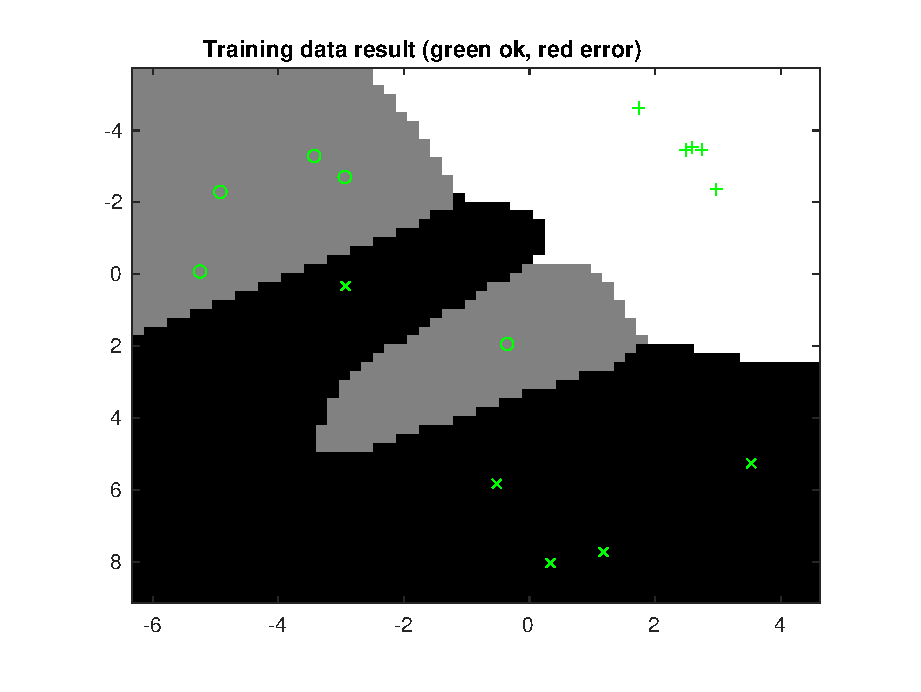
\includegraphics[height=4cm]{images/overfit_result_train}
\caption{Results of a multilayered neural network in a reduced version of the training set 3.}
\label{fig:overfit_result_train}
\end{figure}

\begin{figure}[!htb]
\centering
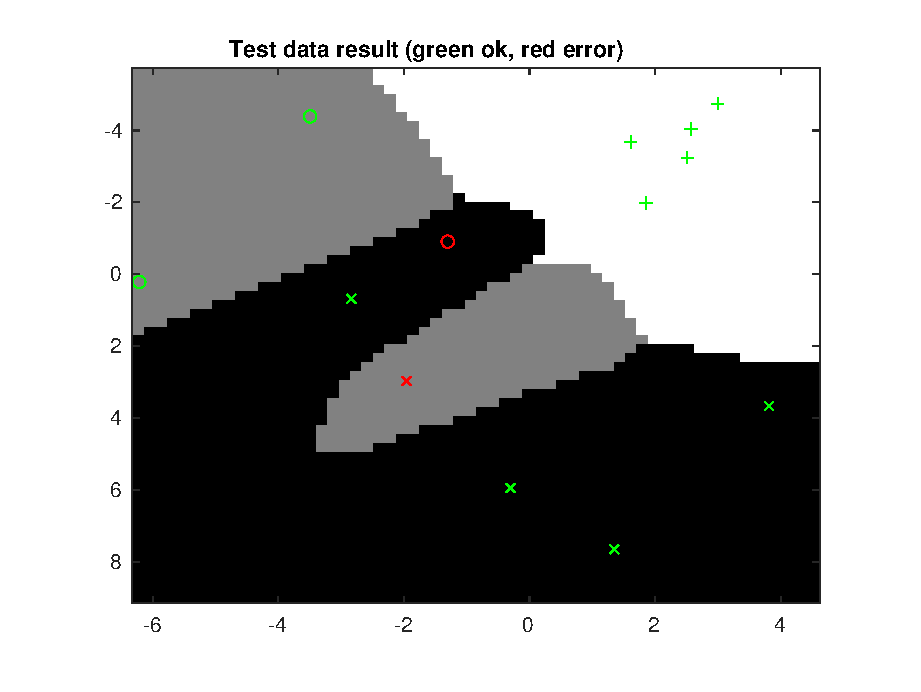
\includegraphics[height=4cm]{images/overfit_result_test}
\caption{Results of a multilayered neural network in a reduced version of the test set 3.}
\label{fig:overfit_result_test}
\end{figure}


\section{Discussion and conclusion}
For the k-NN algorithm, it can be seen that it has a good performance since using the cross validation method the accuracy is above 0.97 for the best k in each dataset. The problem with k-NN is the need of having a huge database (for certain applications) to store all the training data, and the excessive time it takes to perform the comparisons and the calculations of the distances.

The backpropagation algorithm with one layer is simple, fast and have good results with linearly separable datasets. The results are mediocre in other cases, but something good about this technique is that it scales to two layers and more samples, achieving performance close to k-NN with a fraction of the computational cost (after training). With more layers, more complex input and more samples, the performance would be better than in k-NN.

\end{document}
